%======================================================================
\chapter{Theoretical framework}\label{ch2:Theoframework}

\markright{Theoretical framework}
%======================================================================


\section{Soft Colloids}

\paragraph{What is a colloid?} A colloid is a many-body system composed of tiny\footnote{nanometer to micrometer sized} particles, typically named colloids, dispersed in a continuum medium called solvent. 
This model is used to represent physical phenomena such as equilibrium\footnote{such as gas, liquid, solid} and non-equilibrium phase states\footnote{gels, glasses}, as well as to construct effective interaction potentials in many-body systems and to explore the mechanical response of materials.
Also serves as an introductory guido to the physics of dispersions, emulsions, pastes, paints, polymers, gels, and liquid crystals, granular media and living cells and tissues\citep{castanedapriegoColloidalSoftMatter2021,yunkerPhysicsOrderedDisordered2014}.

\paragraph{Why colloids are used} The main features of the colloidal model are that they are relatively slow, typical around \SI{1}{\micro\second} to \SI{1}{\second}, allowing to observe the dynamics in real time.
The interaction between the particles are of the order of the thermal energy.
They can be studied on a single-particle level by means of different complementary techniques\citep{castanedapriegoColloidalSoftMatter2021,yunkerPhysicsOrderedDisordered2014}. 
This features allow to use mathematical tool such as brownian motion or molecular dynamics to analyze the systems with computer simulations and mathematical analysis, also to be easily observed and tracked via optical microscopy.

\paragraph{what is soft colloid} Now that we have a general understanding of the concept of colloids, we will explore the concept of soft colloids.
There are a variety of explanations to softenss: particle elasticity, diversity of particle interactions, and particle volume fraction.
The particle elasticity represents the ratio of the elastic free energy $\Delta F$ with the thermal energy $kT$\footnote{
\begin{gather}
    \epsilon = \frac{\Delta F}{kT}.
\end{gather}
}
In contrast, the softness explain by particle interactions is characterized by the form of the repulsive pair potential between two particles.
Finally, the particle volume fraction contributes to the ability of the particles to deform or compress, in contrast to hard spheres\footnote{The patchy particles are hard spheres, but the hydrogel network is a soft ``particle''}\citep{vlassopoulosTunableRheologyDense2014}.


\section{Mechanical response}


Rheological properties of concentrated dispersions strongly depend on the microstructure, which not only depends on the interaction potential but also on the size distribution of the particles\citep{senffTemperatureSensitiveMicrogel1999}.


\section{Hydrogels}

\subsection{Gels}

\paragraph{Gel point} For any polymer network formation, a critical point exists at which the reaction phase transitions from liquid to solid. 
This point is referred to as the gel point.
Although gelation is not the focus of the research, the ``gel point'' is a crucial concept that demonstrates how certain characteristics can be shared.
At this point, many properties of the polymer networks change abruptly, and the properties that are more useful for applications can be reached beyond the gel point.
Consequently, numerous theoretical models\footnote{The classical approches to predict the relationship between gelation and the extent of reaction in step-growth polymerzation are the Carothers model and Flory-Stockmayer\citep{guPolymerNetworksPlastics2020}.} have been developed to predict the gel point for various network formation processes, including mean-field theory, critical percolation theory, and the kinetic gelation model\citep{guPolymerNetworksPlastics2020}.

\paragraph{Gels} Once the polymer network exceeds its gelation point, gels can be described as polymer networks that form through crosslinks or supramolecular bonds. 
These gels can become swollen in liquid media, such as water or organic solvents.
The network structure guarantees that the liquid is retained within the material.
Gels generally display Young's moduli within the range of 103–104 Pa, yet they often exhibit the capacity for significant deformation.
Examples of gels include gelatin, fibrin, and polyacrylamide hydrogel\citep{guPolymerNetworksPlastics2020}.


\paragraph{Microgels}  
Microgel particles consist of crosslinked macromolecules of colloidal size that swell in the solvent. 
The particle interaction potential strongly depends on the crosslinking density, and microgels exhibit a behavior ranging from that of polymer solutions to that of hard spheres. 
At intermediate degree of crosslinking and swelling the microgels start to resemble the behavior of multiarm star polymers or block copolymer micelles\citep{senffTemperatureSensitiveMicrogel1999}.


\paragraph{Hydrogels}
In the swollen state of the gel, most of the water is in a “free” state and can freeze at the usual freezing point. 
However, some water molecules which are associated with the polymeric chains of the gel network cannot freeze at the usual freezing point. 
This water is called “bound water”\citep{lelePredictionsBoundWater1997}.

Water is bound to the polymer chains through hydrogen-bonding associations and through physical (hydrophobic) interactions\footnote{The total bound water content (BWC) can be calculated from the ratio of total number of polymer-water contacts in the gel to the number of polymer-water contacts per molecule of bound water.}\citep{lelePredictionsBoundWater1997}. 

Hydrogels are tunable soft and aqueous gels\citep{bonyadiReviewFrictionLubrication2020}.


\paragraph{Argument} Why we can use a simulation protocol for microgels to modeled hydrogels?




\subsection{Cross-linking mechanisms}

\paragraph{Intro to cross linking}
A crosslinker is a molecule that functions as a bridge between polymer chains, thereby facilitating the formation of an interconnected network.
As previously suggested, it is pertinent to understand the mechanisms of crosslinking in order to gain insight into the correlation between these mechanisms and mechanical properties, such as elasticity, viscosity, solubility, glass transition temperature, strength, toughness, and melting point stiffness, swelling capacity, viscosity, and so forth\citep{priyaComprehensiveReviewHydrogel2024}.
The elements under consideration form stable bonds, which are comonly categorized into two main types: covalent (permanent) and physical (reversible)\citep{bustamantetorresHydrogelsClassificationAccording2021}.
However, recent mechanisms, such as mechanical crosslinker mechanics, have been demostrated to form bridges due to the topology of the constituents of the hydrogel.

\begin{figure}[!ht]
    \centering
    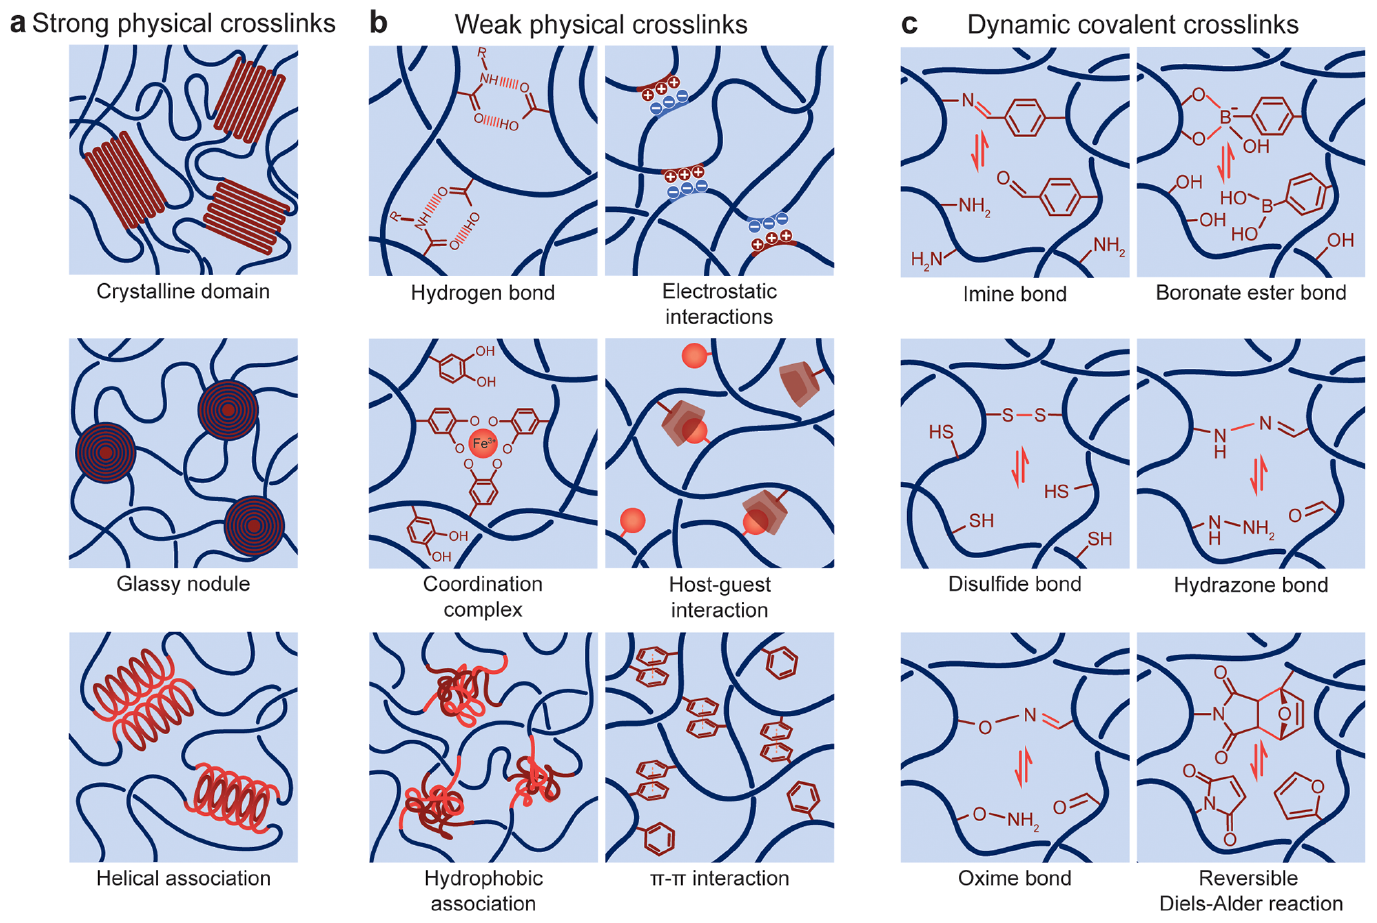
\includegraphics[width=0.8\textwidth]{figs/crosslinker_mechanisms.png}
    \caption{Image with the three different crosslinker mechanisms}
\end{figure}


\paragraph{Difference between physical and chemical bonds}
Although the concept of bonding is central to comprehending chemical structures and reactions.
The criteria employed to characterize a chemical bond, its physical origin, and its nature remain subjects of debate\citep{kumarDevelopingCriterionCharacterize2021}.
Consequently, establishing a precise distinction between ``covalent'' and ``non-covalent'' bonds remains challenging.
Therefore, the description of crosslinker mechanisms is limited to the principal interactions reported in articles and the synthesis process, rather than focusing on the classification of interactions as ``covalent'' or ``non-covalent'', but rather as ``reversible'' or ``irrevarsible''.
Also in the recent work \citep{picchioniHydrogelsBasedDynamic2018} it is shown a ``covalent'' reversible network. 
Nonetheless, a general consensus exists that non-covalent bonds are, as a rule, recognized as being weaker than covalent bonds and it is widely accepted that a distinguishing characteristic between covalent and noncovalent bonds is the energy of interaction and equilibrium bond distance\citep{kumarDevelopingCriterionCharacterize2021,novikovNonCovalentInteractionsPolymers2023}.

\begin{figure}[!ht]
    \centering
    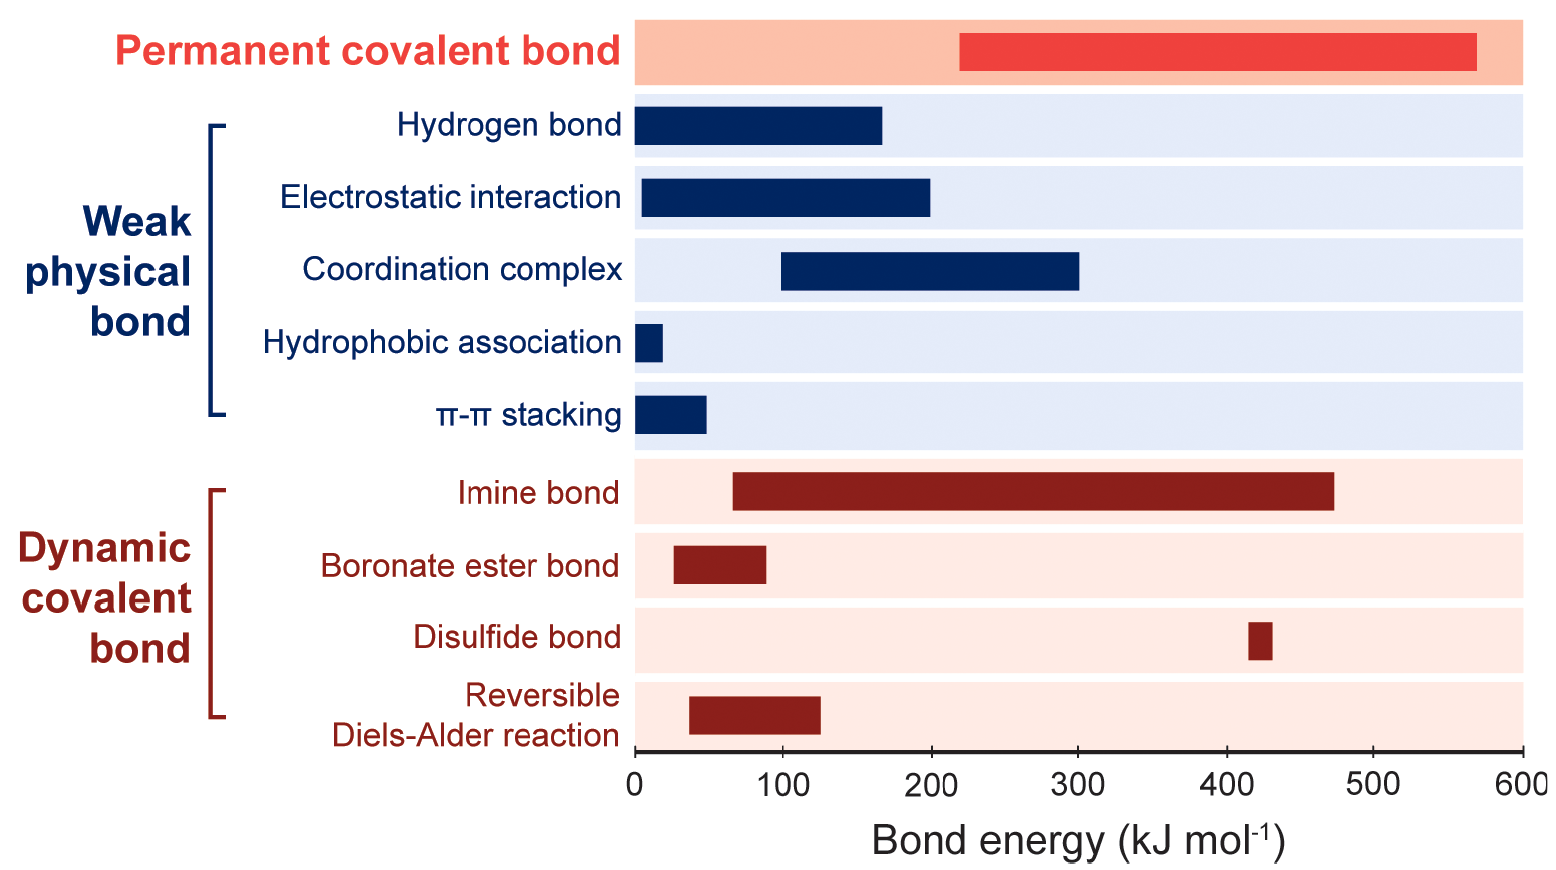
\includegraphics[width=0.8\textwidth]{figs/bonds_energy.png}
    \caption{Bond energies of various types of permanent covalent crosslinks, weak physical cross-links, and dynamic covalent crosslinks.}
\end{figure}

\paragraph{Irreversible Cross-linking}
In irreverisble cross-linked hydrogels, polymer chains are synthesized by chain growth polymerization, graft copolymerization, addition and condensation polymerization, ezymatic method, reactive functions groups and gamma and electron beam polymerization\citep{maitraCrosslinkingHydrogelsReview2014,bustamantetorresHydrogelsClassificationAccording2021}.
This types of crosslinking mechanisms exhibit a high degree of strength and stability, leading to a structural arrangement of interconnected polymer chains that is more robust and resistant to alterations in environmental conditions, such as temperature and pH\citep{maitraCrosslinkingHydrogelsReview2014}.


\paragraph{Reversible Cross-linking}
In reversible cross-linked hydrogels, polymer chains are held together by molecular entanglements or physicochemical interactions, including van der Waals forces, hydrogen bonds, hydrophobic interactions, charge condensation, crystallite formation, and supramolecular chemistry\citep{bustamantetorresHydrogelsClassificationAccording2021,maitraCrosslinkingHydrogelsReview2014}.
Some of the syhtesis methods for reverisble crosslinkin mechanisms are ionic interaction, crystallization, stereocomplex formation, hydrophobized polysaccharides, protein interaction, amphilic copolymers and hydrogen bond\citep{maitraCrosslinkingHydrogelsReview2014,bustamantetorresHydrogelsClassificationAccording2021}.
Furthermore, molecular reversibility can be actually achieved in two different ways: either by making use of equilibrium reactions (e.g., the Diels-Alder one) or through dynamic exchange reactions (e.g., reaction of an excess amino groups with epoxide ones)\citep{picchioniHydrogelsBasedDynamic2018}. 


\paragraph{Mecanical bonds}
As previously mentioned, a novel class of polymer architecture has recently emerged within the field of polymer science kwnon as mechanically interlocked polymers (MIPs). 
These polymers are distinguished by the presence of a mechanical bond, that is, a constraint of two (or more) molecular components in space without the formation of covalent bonds\citep{hartMaterialPropertiesApplications2021}.
While these types of hydrogels exhibit substantial conformational flexibility while preserving a persistent spatial correlation between their components, their synthesis remains challenging.

\subsection{Mechanical properties}

[Covalent and non covalent cross linking]
More recently, shear-thinning hydrogels were developed that  are formed through dynamic and reversible cross-linking.34 
For example, physical hydrogels use noncovalent interactions (e.g., supramolecular chemistries) between soluble building blocks in order to self-assemble into a dynamic, reversibly cross-linked  network.35,36 
Likewise, reversible covalent cross-linking strategies can yield dynamic networks with similar properties.37,38 These “dynamic hydrogels” assembled through reversible cross-links afford the unique property of being injectable even after having formed a gel, due to their shear-thinning and selfhealing behaviors. 
Current research on dynamic hydrogels has revealed novel and useful capabilities that have opened new frontiers for this technology. 
For example, they can stabilize delicate protein and cellular cargoes to combat pharmaceutical  cold-chain limitations,39 they can adhere strongly to tissues to  form protective barriers and bandages,40 and they can be delivered through spray applications to coat complex biological  geometries.41\citep{correaTranslationalApplicationsHydrogels2021}

[Like a transition but I don't know]
While dynamic hydrogels are opening up new translational possibilities, significant progress is also being made to introduce unprecedented levels of functionality into biomaterials. 
This includes features such as nanoscale patterning of  bioactive molecules,42,43 programmable drug release,44,45 and  stimuli-responsive behaviors.46,47\citep{correaTranslationalApplicationsHydrogels2021} 

As a consequence, much of the research in this space is trending toward increasingly interdisciplinary projects that recruit the expertise of nanotechnologists, chemists, protein engineers, and synthetic biologists to develop sophisticated multifunctional hydrogels\citep{correaTranslationalApplicationsHydrogels2021}. 


dynamic hydrogels, which can seamlessly transition back and forth from solid like to liquid like during injection thanks to their shear thinning and self healing capabilities. 
These materials, which are gelled within the syringe before injection, additionally have the ability to stabilize drugs over broad temperature ranges and maintain homogeneously mixed  cell solutions.68 70\citep{correaTranslationalApplicationsHydrogels2021} 



\paragraph{General mechanical properties of the croslsinking}
Eventhough, physical crosslinking mechanisms are weaker than chemical ones, there numerous interactions contribute to complex behaviors.
Meanwhile chemical crosslinking mechanisms are easier to control than physical crosslinking mechanisms because their preparation is independent of pH\citep{bustamantetorresHydrogelsClassificationAccording2021} and they are very brittle due to structural inhomogeneity and lack of energy dissipation\citep{xuRoleChemicalPhysical2018}.


\paragraph{Reversible crosslinking}
The aforementioned interactions enable hydrogels to undergo structural changes without the rupture of any covalent bonds. 
Consequently, these materials exhibit enhance responsiveness to external stimuli, such as temperature, pH, or ionic strength. 
Additionally, hydrogels demonstrate high water sensitivity and thermal reversibility\citep{bustamantetorresHydrogelsClassificationAccording2021,priyaComprehensiveReviewHydrogel2024}.
These materials are known to exhibit distinctive properties, including ``self-healing'' behavior, where the gel can reform after being broken.
The lifespan of these hydrogels is brief, ranging from a few days to a maximum of a month, when maintained within physiological media.


\paragraph{Ir-reversible croslsinkg}
Consequently, chemically cross-linked hydrogels generally exhibit greater mechanical strength and long-term stability.  
Furthermore, it generally contains regions of the high cross-linking density and low degree of swelling (clusters), dispersed in the regions of the low cross-linking density and high swelling index due to the hydrophobic aggregation of the cross-linking agent\citep{bustamantetorresHydrogelsClassificationAccording2021}..


\paragraph{Network-mechanical response relation} Introduce the idea of how by understanding the network we can manipulate/control the mechanical response.

The research of hydrophilic polymers has been complex because the physical properties of solubility or swellability depend on different factors, such as the type of polymer, molecular weight, the ratio of polar groups, and degree of cross-linking\citep{bustamantetorresHydrogelsClassificationAccording2021}.
High molecular weight and a high degree of cross-linking will reduce the hydrophilicity of the molecule [18,19]\citep{bustamantetorresHydrogelsClassificationAccording2021}.


\section{Molecular Dynamics}

\subsection{Langevin dynamics}

From a general point of view there are two types of methods to make a quatitative description of systems: one focused on simulating dynamics at the microscale, and the other dedicated to deriving or establishing evolutionary equations at the macroscale\citep{wangMultiscaleModelingSimulation2025}.
Since the assumption is made that the mechanical response of a hydrogel is predominantly derived from its internal structure\footnote{Poner citas que desmuestrén que no es hipótesis, si no que se sabe} we choose to simulate the dynamics at the microscale.
Additionally, by treating the hyrogel as a colloid, permits applying molecular dynamics to model its response under shear deformation. 
Finally, there are two commonly used mathematical frameworks to model the molecular dynamics, the continuous time random walk (CTRW) model and the Langevin equation\citep{wangMultiscaleModelingSimulation2025}, in this work we decided\footnote{Supongo que eventualmente justificaré la desición.} to use the langevin dynamics mathematical framework.

This is because, the solid phase of the colloid has a large mass and will change their momenta after many collisions with the solvent molecules and the picture which emerges is that of the heavy particles forming a system with a much longer time scale than the solvent molecules\citep{Thijssen2007} and Langevin theory takes advantage of this difference in time scale to eliminate the details of the degrees of freedom of the solvent particles and represent their effect by stochastic and dissipative forces allowing longer simulations that would be impossible if the solvent were explicitly included\citep{pastorTechniquesApplicationsLangevin1994}.
However, the representation of the solvent by a stochastic and dissipative force, introduce the problem of characterize two very different timescales, one associated with the slow relaxation of the initial velocity of the brownian particle and another linked to the frequent collisions that the brownian particle suffers with particles of the bath\citep{tsl2006}\footnote{Para traer a colación la sensibilidad de la respuesta mecánica al parámetro de damp.}. 
Therefore, two terms are used to create a mathematical representation of the solvent: a frictional force proportional to the velocity of the particle and a fluctuating force. 
Hence,
\begin{gather}
    m\dv{\vec{v}(t)}{t}=\vec{F}(t)-m\gamma\vec{v}(t)+\vec{R}(t).\label{eqn:BrownianDyn1}
\end{gather}
The friction constant $\gamma$\footnote{Cuidado con las unidades. Hacer análisis dimensional, porque por la condición de correlación en $R$, $\gamma$ ocupa tener unidades de masa entre tiempo, pero en la ecuación, solo ocupa unidades de $1/s$.} parametrises the effect of solvent damping and activation and is commonly referred to as the collision frequency in the simulation literature, even though formally a Langevin description implies that the solute suffers an infinite number of collisions with infinitesimally small momentum transfer.
Also, the fact that the second term is not a function of the position of any of the particles involves the neglect of hydrodynamic interaction or spatial correlation in the friction kernel spatial correlation in the friction kernel\citep{pastorTechniquesApplicationsLangevin1994}.
On the other hand, $\vec{R}(t)$\footnote{No me acuerdo en donde está que se puede asumir que tiene distribución gaussiana.} is a ``random force'' subject to the following conditions
\begin{align*}
    \expval{\vec{R}(t)} &= 0 \\
    \expval{\vec{R}(t)\vec{R}(t')} &= 2k_{B}T\gamma\delta\qty(t-t') 
\end{align*}
The no time correlation is equivalent to assuming that the viscoelastic relaxation of the solvent is very rapid with respect to solute motions\footnote{Grote land Hynes [26] have investigated this assumption for motions involving barrier crossing and have found that while it is seriously in error for passage over sharp barriers (such as 12 recombination); it is quite adequate for conformational transitions such as might be found in polymer motions.\citep{pastorTechniquesApplicationsLangevin1994}}.

In comparing the results of Langevin dynamics with those of other stochastic methods [28-31], the relevant variable is the velocity relaxation time, $\tau_{v}$ which equals $\gamma^{-1}$\citep{pastorTechniquesApplicationsLangevin1994}
The Langevin equation improves conformational sampling over standard molecular dynamics\citep{paquetMolecularDynamicsMonte2015}.

\begin{itemize}
    \item Hablar acerca de que la fuerza aleatoria puede tener distribución gaussiana, pero no necesariamente.
    \item hablar de la ecuación de Green-Kubo: \[\eta=\frac{V}{k_B T}\int_{0}^{\infty}\expval{\sigma_{xy}(t)\sigma_{xy}(0)}\mathrm{d}t\]
    \item No se que tanto hablar de la idea de correlación y su aplicación en estos temas.
\end{itemize}

\subsection{Velocity Verlet}

L Verlet. Computer” experiments” on classical fluids. I. Thermodynamical properties of Lennard-Jones molecules. Physical Review, 159(1):98103, 1967.

J. M. Haile. Molecular Dynamics Simulation: Elementary Methods.  John Wiley \& Sons, Inc., New York, NY, USA, 1st edition, 1992.

Richard L. Burden and J. Douglas Faires. Numerical Analysis. Brooks  Cole, 8 edition, 12 2008.

Molecular Dynamics, Method For, and Microscale Heat Transfer. Molecular Dynamics Method. Bioinformatics, 2(Md):189–226, 2000.

Shichi Nose. A molecular dynamics method for simulations in the canonical ensemble. Molecular Physics, 52(2):255–268, 1984.

M Tuckerman, B J Berne, and G J Martyna. Reversible multiple time  scale molecular dynamics. The Journal of Chemical Physics, 97(3):1990,  1992.

\subsection{How to compute stres sin molecular dynamics}

%To characterize the behaviour of materials, constitutive relations serve as an input to the continuum theory\dots\footnote{Capaz e ir introduciendo ideas del Clausius\citep{clausiusXVIMechanicalTheorem1870}}

\paragraph{Motivation: Molecular stress is equivalent to continuum stress} \dots This derivation can be found in the apendix of\citep{admalUnifiedInterpretationStress2010}\footnote{Describe more if what is done in this article}.\footnote{(Eventualmente pondré esto en párrafo) Notation:
    $\bm{\sigma}$ Tensor, $\vec{\sigma}$ vector, $\sigma_{i,j}$ tensor, $\overline{\sigma}$ time average, 
}
Consider a system of $N$ interacting particles with each particle position given by
\begin{equation}
    \vec{r}_{\alpha} = \vec{r} + \vec{s}_{\alpha}\label{eqn:DerVirTen1},
\end{equation}
where $\vec{r}$ is the position of the center of mass of the system and $\vec{s}_\alpha$ is the position of each point relative to the center of mass.
Hence, we can express the momentum of each particle as
\begin{equation}
    \vec{p}_\alpha = m_\alpha\qty(\dot{\vec{r}}+\dot{\vec{s}}_\alpha) = m_\alpha\qty(\dot{\vec{r}}+\vec{\upsilon}_\alpha^{\mathrm{rel}}).\label{eqn:DerVirTen2}
\end{equation}
Before starting the procedure, lets take into account that the center of mass of the system is given by
\begin{equation}
    \vec{r} = \frac{\sum_{\alpha}m_\alpha\vec{s}_\alpha}{\sum_{\alpha}m_\alpha}\label{eqn:DerVirTen3},
\end{equation}
and by replacing~\eqref{eqn:DerVirTen1} in~\eqref{eqn:DerVirTen2} we get the following relations, which will be used later,
\begin{equation}
    \sum_\alpha m_\alpha\vec{r}_\alpha = \vec{0},\quad
    \sum_\alpha m_\alpha\vec{\upsilon}_\alpha^{\mathrm{rel}} = \vec{0}.\label{eqn:DerVirTen4}
\end{equation}

Now we can start by computing the time derivative of tensorial product $\vec{r}_\alpha\otimes\vec{p}_\alpha$\footnote{It is interesting to note that the tensorial product $\vec{r}_\alpha\otimes\vec{p}_\alpha$ has units of action and by tacking the time derivative we are dealing with terms that has units of energy.
},
\begin{equation}
    \dv{t}\qty(\vec{r}_\alpha\otimes\vec{p}_\alpha) = 
    \underbrace{\vec{\upsilon}_\alpha^{\mathrm{rel}}\otimes\vec{p}_\alpha}_{\mathrm{Kinetic~term}} 
        +
        \underbrace{\vec{r}_\alpha\otimes\vec{f}_\alpha}_{\mathrm{Virial~term}},\label{eqn:DerVirTen5}
\end{equation}
which is known as the \textit{dynamical tensor virial theorem} and it is simply an alternative form to express the balance of linear momentum.
This theorem becomes useful after making the assumption that there existis a time scale $\tau$, which is short relative to macroscopic processes but long relative to the characteristic time of the particles in the system, over which the particles remain close to their original positions with bounded positions and velocities.
Taking advantage of this property we can compute the time average of~\eqref{eqn:DerVirTen5},
\begin{equation}
    \frac{1}{\tau}\qty(\vec{r}_\alpha\otimes\vec{p}_\alpha)\bigg|_{0}^{\tau} = 
    \overline{\vec{\upsilon}_\alpha^{\mathrm{rel}}\otimes\vec{p}_\alpha} 
        +
    \overline{\vec{r}_\alpha\otimes\vec{f}_\alpha}.\label{eqn:DerVirTen6}
\end{equation}
Assuming that $\vec{r}_\alpha\otimes\vec{p}_\alpha$ is bounded, and the time scales between microscopic and continuum processes are large enough, the term on the left-hand side can be as small as desired by tacking $\tau$ sufficiently large and by summing over all particles we achieve the \textit{tensor virial theorem}:
\begin{equation}
    \overline{\mathbf{W}} = -2\overline{\mathbf{T}},\label{eqn:DerVirTen7}
\end{equation}
where
\begin{equation}
    \overline{\mathbf{W}} = \sum_\alpha\overline{\vec{r}_\alpha\otimes\vec{f}_\alpha}\label{eqn:DerVirTen8}
\end{equation}
is the time-average virial tensor and
\begin{equation}
    \overline{\mathbf{T}}=\frac{1}{2}\sum_\alpha\overline{\vec{\upsilon}_\alpha^{\mathrm{rel}}\otimes\vec{p}_\alpha}\label{eqn:DerVirTen9}
\end{equation}
is the time-average kinetic tensor.
This expression for the tensor virial theorem applies equally to continuum systems that are not in macroscopic equilibrium as well as those that are at rest.

The assumption of the difference between the time scales allow us to simplify the relation by replacing~\eqref{eqn:DerVirTen2} in~\eqref{eqn:DerVirTen9}, so that,
\begin{equation}
    \overline{\mathbf{T}}=
        \frac{1}{2}\sum_\alpha m_\alpha\overline{\vec{\upsilon}_\alpha^{\mathrm{rel}}\otimes\vec{v}_\alpha^{\mathrm{rel}}}
        +
        \frac{1}{2} \left[\overline{\sum_\alpha m_\alpha\vec{\upsilon}_\alpha^{\mathrm{rel}}}\right]\otimes\dot{\vec{r}}\label{eqn:DerVirTen10},
\end{equation}
which is not the simplification we expected, however, by the relations from~\eqref{eqn:DerVirTen4}, equation~\eqref{eqn:DerVirTen10} simplifies to\footnote{No estoy muy seguro si incluir una discusión acerca del término cinético en la expresión del virial. Posiblemente un párrafo\dots posiblemente lo ponga en la interpretación del teorema.
También, no se si ir metiendo interpretación durante la derivación o no, pero bueno.}
\begin{equation}
    \overline{\mathbf{T}}=
        \frac{1}{2}\sum_\alpha m_\alpha\overline{\vec{\upsilon}_\alpha^{\mathrm{rel}}\otimes\vec{\upsilon}_\alpha^{\mathrm{rel}}}\label{eqn:DerVirTen11}.
\end{equation}
On the other hand, instead of reducing the expression, we start to create the conection with the Cauchy stress tensor by distributing~\eqref{eqn:DerVirTen8} into an internal and external contributions,
\begin{equation}
    \overline{\mathbf{W}} = 
    \underbrace{\sum_\alpha\overline{\vec{r}_\alpha\otimes\vec{f}_\alpha^{\mathrm{int}}}}_{\overline{\mathbf{W}}_{\mathrm{int}}}
        +
        \underbrace{\sum_\alpha\overline{\vec{r}_\alpha\otimes\vec{f}_\alpha^{\mathrm{ext}}}}_{\overline{\mathbf{W}}_{\mathrm{ext}}}.\label{eqn:DerVirTen12}
\end{equation}
The time-average internal virial tensor takes into account the interaction between particle $\alpha$ with the other particles in the system, meanwhile, the time-average external virial tensor considers the interaction with atoms outside the system, via a traction vector $\vec{t}$ and external fields acting on the system represented by $\rho\vec{b}$, where $\rho$ is the mass density of it and $\vec{b}$ is the body force per unit mass applied by the external field.
Therefore we can express the following,
\begin{equation}
    \sum_\alpha\overline{\vec{r}_\alpha\otimes\vec{f}_\alpha^{\mathrm{ext}}}
    :=
    \int_{\delta\Omega}\vec{\xi}\otimes\vec{t}dA 
    +
    \int_{\Omega}\vec{\xi}\otimes\rho\vec{b}dV.\label{eqn:DerVirTen13}
\end{equation}
Where $\vec{\xi}$ is a position vector within the domain $\Omega$ occupied by the system of particles with a continuous closed surface $\delta\Omega$.
Assuming that $\Omega$ is large enough to express the external forces acting on it in the form of the continuum traction vector $\vec{t}$.

With this we can substitute the traction vector with $\vec{t}=\bm{\sigma}\vec{n}$, where $\bm{\sigma}$ represent the Cauchy stress tensor and applying the divergence theorem in~\eqref{eqn:DerVirTen13}, we have 
\begin{equation}
    \overline{\mathbf{W}}_{\mathrm{ext}}
     =\int_{\Omega}
        \left[
            \vec{\xi}\otimes\rho\vec{b}+\mathrm{div}_{\vec{\xi}}\qty(\vec{\xi}\otimes\bm{\sigma})
        \right]dV
        =
    \int_{\Omega}
        \left[
            \bm{\sigma}^{\mathrm{T}}
            +
            \vec{\xi}\otimes\qty(\mathrm{div}_{\vec{\xi}}\bm{\sigma}+\rho\vec{b})
        \right]dV\label{eqn:DerVirTen14}
\end{equation}
Since we assume that we are under equilibrium conditions, the term $\mathrm{div}_{\vec{\xi}}\bm{\sigma}+\rho\vec{b}$ is zero~\eqref{eqn:DerVirTen14} it simplifies to
\begin{equation}
    \overline{\mathbf{W}}_{\mathrm{ext}}
    =V\bm{\sigma}^{\mathrm{T}}\label{eqn:DerVirTen15}.
\end{equation}
By tacking into account that we integrate over the domain $\Omega$ we can say that we compute the spatial average of the Cauchy stress tensor,
\begin{equation}
    \bm{\sigma}_{\mathrm{av}} =\frac{1}{V}\int_\Omega\bm{\sigma}dV\label{eqn:DerVirTen16},
\end{equation}
in which $V$ is the volume of the domain $\Omega$.
Replacing~\eqref{eqn:DerVirTen15} into~\eqref{eqn:DerVirTen12}, the tensor virial theorem~\eqref{eqn:DerVirTen7} can be expressed as,
\begin{equation}
    \sum_\alpha\overline{\vec{r}_\alpha\otimes\vec{f}_\alpha^{\mathrm{int}}}
    +
    V\bm{\sigma}_{\mathrm{av}}^{\mathrm{T}}
    =
    -\sum_\alpha m_\alpha\overline{\vec{\upsilon}_\alpha^{\mathrm{rel}}\otimes\vec{\upsilon}_\alpha^{\mathrm{rel}}}.\label{eqn:DerVirTen17}
\end{equation}
Finally, solving for the Cauchy Stress tensor we get,
\begin{equation}
    \bm{\sigma}_{\mathrm{av}}
    =
    -\frac{1}{V}
    \left[
        \sum_\alpha\overline{\vec{f}_\alpha^{\mathrm{int}}\otimes\vec{r}_\alpha}
        +
        \sum_\alpha m_\alpha\overline{\vec{\upsilon}_\alpha^{\mathrm{rel}}\otimes\vec{\upsilon}_\alpha^{\mathrm{rel}}}
    \right],\label{eqn:DerVirTen18}
\end{equation}
an expression that describe the macroscopic stress tensor in terms of microscopic variables\footnote{It is important to acknowledge that several mathematical subtleties were not taken into consideration, however all the mathematical formality is adressed by Nikhil Chandra Admal and E. B. Tadmor in~\citep{admalUnifiedInterpretationStress2010}}.

To end the section it is important to show that~\eqref{eqn:DerVirTen18} is symmetric.
Therefore, we rewrite the internal force as the sum of forces between the particles,
\begin{equation}
    \vec{f}^{\mathrm{int}}_\alpha = \sum_{{\beta}_{\beta\neq\alpha}}\vec{f}_{\alpha\beta}\label{eqn:DerVirTen19},
\end{equation}
and substituting~\eqref{eqn:DerVirTen19} into~\eqref{eqn:DerVirTen18}, we have
\begin{equation}
    \bm{\sigma}_{\mathrm{av}}
    =
    -\frac{1}{V}
    \left[
        \sum_{{\alpha,\beta}_{\beta\neq\alpha}}\overline{\vec{f}_{\alpha\beta}\otimes\vec{r}_\alpha}
        +
        \sum_\alpha m_\alpha\overline{\vec{\upsilon}_\alpha^{\mathrm{rel}}\otimes\vec{\upsilon}_\alpha^{\mathrm{rel}}}
    \right].\label{eqn:DerVirTen20}
\end{equation}
Due to the property $\vec{f}_{\alpha\beta}=-\vec{f}_{\beta\alpha}$ we obtain the following identity
\begin{equation}
    \sum_{{\alpha,\beta}_{\beta\neq\alpha}}\vec{f}_{\alpha\beta}\otimes\vec{r}_\alpha 
    =
    \frac{1}{2}\sum_{{\alpha,\beta}_{\beta\neq\alpha}}\left(\vec{f}_{\alpha\beta}\otimes\vec{r}_\alpha+\vec{f}_{\beta\alpha}\otimes\vec{r}_\beta\right)
    =
    \frac{1}{2}\sum_{{\alpha,\beta}_{\beta\neq\alpha}}\vec{f}_{\alpha\beta}\otimes\left(\vec{r}_\alpha-\vec{r}_\beta\right).\label{eqn:DerVirTen21}
\end{equation}
Therefore, by replacing the identity of~\eqref{eqn:DerVirTen21} into~\eqref{eqn:DerVirTen20}, we have
\begin{equation}
    \bm{\sigma}_{\mathrm{av}}
    =
    -\frac{1}{V}
    \left[
        \frac{1}{2}
        \sum_{{\alpha,\beta}_{\beta\neq\alpha}}\overline{\vec{f}_{\alpha\beta}\otimes\left(\vec{r}_\alpha-\vec{r}_\beta\right)}
        +
        \sum_\alpha m_\alpha\overline{\vec{\upsilon}_\alpha^{\mathrm{rel}}\otimes\vec{\upsilon}_\alpha^{\mathrm{rel}}}
    \right],\label{eqn:DerVirTen22}
\end{equation}
expressed with indexical notation and using the eistein summation convention,
\begin{equation}
    \sigma^{\mathrm{av}}_{ij}
    =
    -\frac{1}{V}
    \left[
        \frac{1}{2}
        \sum_{{\alpha,\beta}_{\beta\neq\alpha}}\overline{f^{\alpha\beta}_{i}r^\alpha_{j} + f^{\beta\alpha}_{i}r^\beta_{j}}
        +
        \sum_\alpha m_\alpha\overline{\upsilon^{\alpha~\mathrm{rel}}_{i}\upsilon^{\alpha{\mathrm{rel}}}_j}
    \right],\label{eqn:DerVirTen23}
\end{equation}
which is the same expression implemented in~LAMMPS\citep{LAMMPS}.\footnote{No se si poner la referencia a la pagina de documentacion\href{https://docs.lammps.org/compute_stress_atom.html}{https://docs.lammps.org/compute\_stress\_atom.html}}




\begin{comment}


\section{Soft colloids}\label{ch2:SoftColloids}


\begin{itemize}
    \item Why we can model hydrogels as Soft colloids?
    \item Idea of patchy particles and insterpretaion of interaction rules
    \item teaser of simulation experiments
\end{itemize}


Hydrophilic gels that are usually referred to as hydrogels are networks of polymer chains that are sometimes found as colloidal gels in which water is the dispersion medium [1]\citep{ahmedHydrogelPreparationCharacterization2015a}.


Ahora no se si la intro solo centrarme en aplicaciones de hidrogeles y poner la discusion de cross link aquí y así.


\subsection{Crosslinking mechanisms}\label{ch1:Cross-linking}

What a low hysteresis means in a hydrogel?

Hydrogels are made up of cross-linked polymer chains. 
The cross-linking creates a three-dimensional network with spaces (pores) between the polymer chains.  
These pores can absorb and hold a significant amount of water, sometimes up to  thousands of times their dry weight. 
The water molecules are retained within the  polymer network, which contributes to the porous nature of hydrogels. 
The polymer chains in hydrogels are flexible, allowing them to stretch and deform under  stress. 
Though hydrogels can be categorized by the types of polymer, cross-linking,  physical appearance, and network electrical charge [31], their common mechanical characteristics are porosity and elasticity. 
These two attributes make hydrogels  highly versatile and useful in various applications, such as in medical devices, drug  delivery systems, and tissue engineering, as discussed above.




\paragraph{Tunnable mechanical response with applications} Review of articles of applications 

Just describe the phenomena and say that it depends on the structure and so on.


\section{Deformation and Stress}

\paragraph{What is stress?} Relation stress-strain.

\paragraph{How we model a material using stress-strain relations} Constitutive equations?

\subsection{Mechanical response}\label{ch2:MechResponse}

\paragraph{Viscoelasticity} An overview with equations.

\paragraph{Yield stress} and overview with equations.

\paragraph{Shear thinning} an overview with equations.


\section{Molecular dynamics}\label{ch2:MD}

\begin{itemize}
    \item Langevin equation
    \item Velocity Verlet
    \item Periodic Boundary Conditions
\end{itemize}


\paragraph{Overview of the method}

\paragraph{Characteristics of the method}


\subsection{Periodic Boundary Conditions}


\end{comment}

\newpage
